\fancychapter{The work}

{\color{red}\bfseries IMPORTANT NOTICE: This chapter should not be called ``The Work'' in the final version of your dissertation. This comment was inserted after some of my faculty collegues noticed that some naive souls call the chapter ``The Work''. This is by no means appropriate. This and all chapter names should be named accordingly to your thesis.}

The third chapter is typically the work you have performed in your thesis. Obviously you should focus on your contributions, but do not forget to write it so that others can understand. Never assume the reader knows the subject (unless it is really obvious). Your work is typically done in a very specific area which others may not know as much. So try to make it as clear as possible; and a self-explaining figure is always a big help.

\begin{figure}[t]
\centering
\subfigure[caption for subfigure a]{\includegraphics[scale=0.65]{images/img1.eps}\label{chp3:img1}}
\hspace*{0.5cm}
\subfigure[caption for subfigure b]{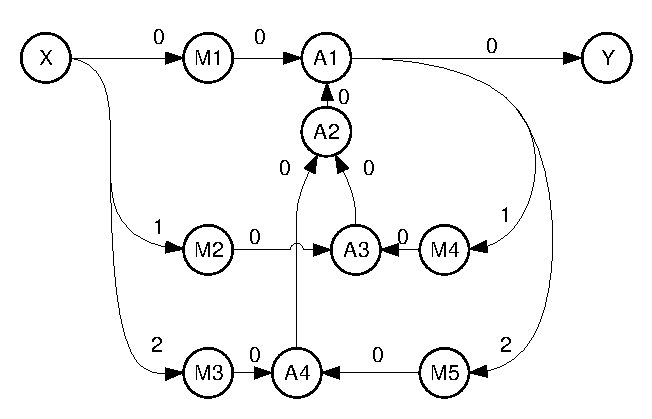
\includegraphics[scale=0.65]{images/img2.eps}\label{chp3:img2}}\\
\caption{A figure example.}
\label{fig:rmain figure}
\end{figure}

See the source code to see how to reference each of the subfigures \ref{chp3:img1} or \ref{chp3:img2}, or the main figure \ref{fig:rmain figure}.

There are several ways to define formulas (see the \textit{Short Math Guide for LaTeX} included in the package). The typical method is to use (see source code): 
\begin{equation}
a= b + c
\end{equation}
or
\begin{align}
c &= d \cdot e \nonumber\\
d &= \mathbf{X}^{\mathsf{T}} \mathbf{Y}+ \gamma e^{2\pi}
\label{chp3:eq1} 
\end{align}
or
\begin{subequations}
\begin{align}
c &= d \cdot e \label{chp3:eq2:a} \\
d &= \mathbf{X}^{\mathsf{T}} \mathbf{Y} + \gamma e^{2\pi}
\label{chp3:eq2:b} 
\end{align}
\label{chp3:eq2} 
\end{subequations}
where $\mathbf{X}$ and $\mathbf{Y}$ are column vectors (you should always present the meaning of each parameter). The \textbf{AMS} packages allow to use the command \verb"\eqref" to cite equations such as \eqref{chp3:eq1},  \eqref{chp3:eq2:a},\eqref{chp3:eq2:b} or \eqref{chp3:eq2} (see source code).

\section{Summary}

It is typical a good ideia to have an ending section summarizing the chapter.

% Ensure that the next chapter starts in a odd page
\cleardoublepage
 
